\documentclass[pdf]{beamer}
\mode<presentation>{}
\usepackage{minted}
\usepackage{tikz}
\usepackage{pgffor} %% gives looping with \foreach
\usepackage[absolute,overlay]{textpos}
\usepackage{lmodern} %% scalable latin characters
\usetikzlibrary{arrows,shapes,backgrounds}
\usepackage{multirow}
\usepackage{listings} %% another package for code related stuff


%% stuff for minted
\definecolor{mintedBg}{rgb}{0.95, 0.95, 0.95}
\definecolor{blockBg}{rgb}{0.6, 0.6, 0.95}
\definecolor{rnaColor}{rgb}{0, 0.6, 0}
\definecolor{cdsColor}{rgb}{0, 0.4, 0.4}
\definecolor{rnaPol}{rgb}{0.8,0,0.8}
\definecolor{ribosomeCol}{rgb}{0.5,0.5,0.1}
\definecolor{protColor}{rgb}{0.6,0,0.6}
%% colours for nucleotides:
\definecolor{dACol}{rgb}{0.5, 0.5, 0}
\definecolor{dCCol}{rgb}{0.8, 0, 0}
\definecolor{dGCol}{rgb}{0, 0.8, 0}
\definecolor{dTCol}{rgb}{0, 0, 0.8}

\definecolor{navy}{rgb}{0, 0, 0.6}
\definecolor{pur}{rgb}{0, 0, 0.6}
\definecolor{pyr}{rgb}{0.6, 0, 0.2}
%% define styles for different codes
\newminted{cpp}{linenos, bgcolor=mintedBg, fontsize=\footnotesize}
%% then use \begin{cppcode}
\newminted{c}{linenos, bgcolor=mintedBg, fontsize=\footnotesize}
\newminted{perl}{linenos, bgcolor=mintedBg, fontsize=\tiny}
\newminted{sh}{linenos, bgcolor=mintedBg, fontsize=\footnotesize,
  language=bash}
\newminted{console}{linenos, bgcolor=mintedBg, fontsize=\footnotesize}

%% a command to define a subheading
\newcommand\subHeading[1]{
  \par\bigskip {\Large\bfseries#1}\par\smallskip
}

%% I detest indentation in footnotes etc, so try this:
\makeatletter
\renewcommand\@makefntext[1]{\noindent\makebox[0em][r]{\@makefnmark}\tiny#1}
\makeatother
%% the makeatletter and makeatother are required to allow me to
%% to change the macro beginning with an @. (though when I call it
%% I don't use the @ ... 

\setlength\parskip{0.5em}
\setlength\parindent{0ex}

%% to have footnotes without references. This from tex.stackexchange.com
\newcommand\blfootnote[1]{%
  \begingroup  %% this makes it a local redefinition
  \renewcommand\thefootnote{}\footnote{#1}%
  \addtocounter{footnote}{-1}  % this adjusts the footnote counter
  \endgroup
}


\title{Implementing (an) algorithm(s) in perl}
\subtitle{structuring data and scripts}
\author{Martin Jakt}

\begin{document}

\begin{frame}
  \titlepage
\end{frame}

\begin{frame}{In general}
  \begin{enumerate}
  \item What is the input data?
    \begin{itemize}
    \item Where do we get it from (from file / command)
    \item How to store the input data
    \end{itemize}
    \pause
  \item How to structure the program?
    \begin{itemize}
    \item Repeated actions (eg. reading a sequence from a file) to functions
    \item Order of events in script
    \end{itemize}
    \pause
  \item What to output?
    \begin{itemize}
    \item Output functions?
    \item STDOUT / specified file
    \end{itemize}
  \end{enumerate}
\end{frame}

\begin{frame}{Sliding alignment of two sequences}
  \begin{figure}[ht]
    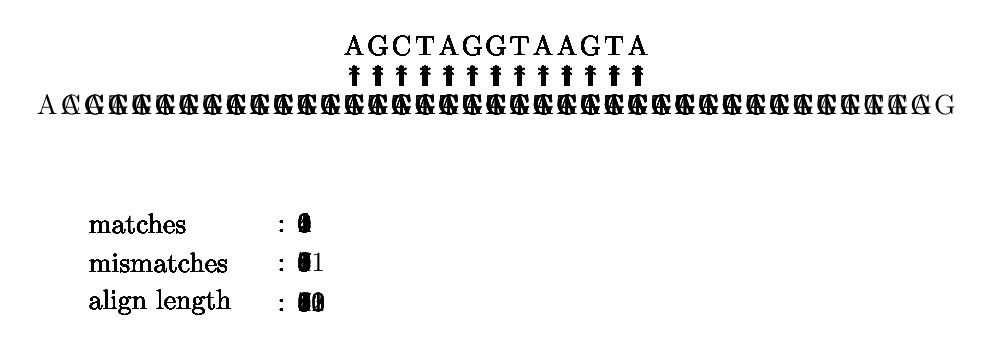
\begin{tikzpicture}[scale=0.5]
      \visible<1>{
	\node  [] (a0) at (0 + 0, 15) {A};
	\node  [] (a1) at (0 + 0.6, 15) {G};
	\node  [] (a2) at (0 + 1.2, 15) {C};
	\node  [] (a3) at (0 + 1.8, 15) {T};
	\node  [] (a4) at (0 + 2.4, 15) {A};
	\node  [] (a5) at (0 + 3, 15) {G};
	\node  [] (a6) at (0 + 3.6, 15) {G};
	\node  [] (a7) at (0 + 4.2, 15) {T};
	\node  [] (a8) at (0 + 4.8, 15) {A};
	\node  [] (a9) at (0 + 5.4, 15) {A};
	\node  [] (a10) at (0 + 6, 15) {G};
	\node  [] (a11) at (0 + 6.6, 15) {T};
	\node  [] (a12) at (0 + 7.2, 15) {A};
	\node [] (b0) at (1.2,13.5) {A};
	\node at (1.2,14.25) {*};
	\node [] (b1) at (1.8,13.5) {C};
	\node at (1.8,14.25) {*};
	\node [] (b2) at (2.4,13.5) {G};
	\node at (2.4,14.25) {*};
	\node [] (b3) at (3,13.5) {T};
	\node at (3,14.25) {*};
	\node [] (b4) at (3.6,13.5) {A};
	\node at (3.6,14.25) {*};
	\node [] (b5) at (4.2,13.5) {G};
	\node at (4.2,14.25) {*};
	\node [] (b6) at (4.8,13.5) {A};
	\draw [line width=2, -] (a8) -- (b6);
	\node [] (b7) at (5.4,13.5) {C};
	\node at (5.4,14.25) {*};
	\node [] (b8) at (6,13.5) {C};
	\node at (6,14.25) {*};
	\node [] (b9) at (6.6,13.5) {T};
	\draw [line width=2, -] (a11) -- (b9);
	\node [] (b10) at (7.2,13.5) {T};
	\node at (7.2,14.25) {*};
	\node [] (b11) at (7.8,13.5) {A};
	\node [] (b12) at (8.4,13.5) {G};
	\node [right] at (-7,10.5) {matches};
	\node [right] at (-2.2,10.5) {: 2};
	\node [right] at (-7,9.5) {mismatches};
	\node [right] at (-2.2,9.5) {: 9};
	\node [right] at (-7,8.5) {align length};
	\node [right] at (-2.2,8.5) {: 11};
}
\visible<2>{
	\node  [] (a0) at (0 + 0, 15) {A};
	\node  [] (a1) at (0 + 0.6, 15) {G};
	\node  [] (a2) at (0 + 1.2, 15) {C};
	\node  [] (a3) at (0 + 1.8, 15) {T};
	\node  [] (a4) at (0 + 2.4, 15) {A};
	\node  [] (a5) at (0 + 3, 15) {G};
	\node  [] (a6) at (0 + 3.6, 15) {G};
	\node  [] (a7) at (0 + 4.2, 15) {T};
	\node  [] (a8) at (0 + 4.8, 15) {A};
	\node  [] (a9) at (0 + 5.4, 15) {A};
	\node  [] (a10) at (0 + 6, 15) {G};
	\node  [] (a11) at (0 + 6.6, 15) {T};
	\node  [] (a12) at (0 + 7.2, 15) {A};
	\node [] (b0) at (-7.8,13.5) {A};
	\node [] (b1) at (-7.2,13.5) {C};
	\node [] (b2) at (-6.6,13.5) {G};
	\node [] (b3) at (-6,13.5) {T};
	\node [] (b4) at (-5.4,13.5) {A};
	\node [] (b5) at (-4.8,13.5) {G};
	\node [] (b6) at (-4.2,13.5) {A};
	\node [] (b7) at (-3.6,13.5) {C};
	\node [] (b8) at (-3,13.5) {C};
	\node [] (b9) at (-2.4,13.5) {T};
	\node [] (b10) at (-1.8,13.5) {T};
	\node [] (b11) at (-1.2,13.5) {A};
	\node [] (b12) at (-0.600000000000001,13.5) {G};
	\node [right] at (-7,10.5) {matches};
	\node [right] at (-2.2,10.5) {: 0};
	\node [right] at (-7,9.5) {mismatches};
	\node [right] at (-2.2,9.5) {: 0};
	\node [right] at (-7,8.5) {align length};
	\node [right] at (-2.2,8.5) {: 0};
}
\visible<3>{
	\node  [] (a0) at (0 + 0, 15) {A};
	\node  [] (a1) at (0 + 0.6, 15) {G};
	\node  [] (a2) at (0 + 1.2, 15) {C};
	\node  [] (a3) at (0 + 1.8, 15) {T};
	\node  [] (a4) at (0 + 2.4, 15) {A};
	\node  [] (a5) at (0 + 3, 15) {G};
	\node  [] (a6) at (0 + 3.6, 15) {G};
	\node  [] (a7) at (0 + 4.2, 15) {T};
	\node  [] (a8) at (0 + 4.8, 15) {A};
	\node  [] (a9) at (0 + 5.4, 15) {A};
	\node  [] (a10) at (0 + 6, 15) {G};
	\node  [] (a11) at (0 + 6.6, 15) {T};
	\node  [] (a12) at (0 + 7.2, 15) {A};
	\node [] (b0) at (-7.2,13.5) {A};
	\node [] (b1) at (-6.6,13.5) {C};
	\node [] (b2) at (-6,13.5) {G};
	\node [] (b3) at (-5.4,13.5) {T};
	\node [] (b4) at (-4.8,13.5) {A};
	\node [] (b5) at (-4.2,13.5) {G};
	\node [] (b6) at (-3.6,13.5) {A};
	\node [] (b7) at (-3,13.5) {C};
	\node [] (b8) at (-2.4,13.5) {C};
	\node [] (b9) at (-1.8,13.5) {T};
	\node [] (b10) at (-1.2,13.5) {T};
	\node [] (b11) at (-0.6,13.5) {A};
	\node [] (b12) at (0,13.5) {G};
	\node at (0,14.25) {*};
	\node [right] at (-7,10.5) {matches};
	\node [right] at (-2.2,10.5) {: 0};
	\node [right] at (-7,9.5) {mismatches};
	\node [right] at (-2.2,9.5) {: 1};
	\node [right] at (-7,8.5) {align length};
	\node [right] at (-2.2,8.5) {: 1};
}
\visible<4>{
	\node  [] (a0) at (0 + 0, 15) {A};
	\node  [] (a1) at (0 + 0.6, 15) {G};
	\node  [] (a2) at (0 + 1.2, 15) {C};
	\node  [] (a3) at (0 + 1.8, 15) {T};
	\node  [] (a4) at (0 + 2.4, 15) {A};
	\node  [] (a5) at (0 + 3, 15) {G};
	\node  [] (a6) at (0 + 3.6, 15) {G};
	\node  [] (a7) at (0 + 4.2, 15) {T};
	\node  [] (a8) at (0 + 4.8, 15) {A};
	\node  [] (a9) at (0 + 5.4, 15) {A};
	\node  [] (a10) at (0 + 6, 15) {G};
	\node  [] (a11) at (0 + 6.6, 15) {T};
	\node  [] (a12) at (0 + 7.2, 15) {A};
	\node [] (b0) at (-6.6,13.5) {A};
	\node [] (b1) at (-6,13.5) {C};
	\node [] (b2) at (-5.4,13.5) {G};
	\node [] (b3) at (-4.8,13.5) {T};
	\node [] (b4) at (-4.2,13.5) {A};
	\node [] (b5) at (-3.6,13.5) {G};
	\node [] (b6) at (-3,13.5) {A};
	\node [] (b7) at (-2.4,13.5) {C};
	\node [] (b8) at (-1.8,13.5) {C};
	\node [] (b9) at (-1.2,13.5) {T};
	\node [] (b10) at (-0.6,13.5) {T};
	\node [] (b11) at (0,13.5) {A};
	\draw [line width=2, -] (a0) -- (b11);
	\node [] (b12) at (0.6,13.5) {G};
	\draw [line width=2, -] (a1) -- (b12);
	\node [right] at (-7,10.5) {matches};
	\node [right] at (-2.2,10.5) {: 2};
	\node [right] at (-7,9.5) {mismatches};
	\node [right] at (-2.2,9.5) {: 0};
	\node [right] at (-7,8.5) {align length};
	\node [right] at (-2.2,8.5) {: 2};
}
\visible<5>{
	\node  [] (a0) at (0 + 0, 15) {A};
	\node  [] (a1) at (0 + 0.6, 15) {G};
	\node  [] (a2) at (0 + 1.2, 15) {C};
	\node  [] (a3) at (0 + 1.8, 15) {T};
	\node  [] (a4) at (0 + 2.4, 15) {A};
	\node  [] (a5) at (0 + 3, 15) {G};
	\node  [] (a6) at (0 + 3.6, 15) {G};
	\node  [] (a7) at (0 + 4.2, 15) {T};
	\node  [] (a8) at (0 + 4.8, 15) {A};
	\node  [] (a9) at (0 + 5.4, 15) {A};
	\node  [] (a10) at (0 + 6, 15) {G};
	\node  [] (a11) at (0 + 6.6, 15) {T};
	\node  [] (a12) at (0 + 7.2, 15) {A};
	\node [] (b0) at (-6,13.5) {A};
	\node [] (b1) at (-5.4,13.5) {C};
	\node [] (b2) at (-4.8,13.5) {G};
	\node [] (b3) at (-4.2,13.5) {T};
	\node [] (b4) at (-3.6,13.5) {A};
	\node [] (b5) at (-3,13.5) {G};
	\node [] (b6) at (-2.4,13.5) {A};
	\node [] (b7) at (-1.8,13.5) {C};
	\node [] (b8) at (-1.2,13.5) {C};
	\node [] (b9) at (-0.600000000000001,13.5) {T};
	\node [] (b10) at (0,13.5) {T};
	\node at (0,14.25) {*};
	\node [] (b11) at (0.6,13.5) {A};
	\node at (0.6,14.25) {*};
	\node [] (b12) at (1.2,13.5) {G};
	\node at (1.2,14.25) {*};
	\node [right] at (-7,10.5) {matches};
	\node [right] at (-2.2,10.5) {: 0};
	\node [right] at (-7,9.5) {mismatches};
	\node [right] at (-2.2,9.5) {: 3};
	\node [right] at (-7,8.5) {align length};
	\node [right] at (-2.2,8.5) {: 3};
}
\visible<6>{
	\node  [] (a0) at (0 + 0, 15) {A};
	\node  [] (a1) at (0 + 0.6, 15) {G};
	\node  [] (a2) at (0 + 1.2, 15) {C};
	\node  [] (a3) at (0 + 1.8, 15) {T};
	\node  [] (a4) at (0 + 2.4, 15) {A};
	\node  [] (a5) at (0 + 3, 15) {G};
	\node  [] (a6) at (0 + 3.6, 15) {G};
	\node  [] (a7) at (0 + 4.2, 15) {T};
	\node  [] (a8) at (0 + 4.8, 15) {A};
	\node  [] (a9) at (0 + 5.4, 15) {A};
	\node  [] (a10) at (0 + 6, 15) {G};
	\node  [] (a11) at (0 + 6.6, 15) {T};
	\node  [] (a12) at (0 + 7.2, 15) {A};
	\node [] (b0) at (-5.4,13.5) {A};
	\node [] (b1) at (-4.8,13.5) {C};
	\node [] (b2) at (-4.2,13.5) {G};
	\node [] (b3) at (-3.6,13.5) {T};
	\node [] (b4) at (-3,13.5) {A};
	\node [] (b5) at (-2.4,13.5) {G};
	\node [] (b6) at (-1.8,13.5) {A};
	\node [] (b7) at (-1.2,13.5) {C};
	\node [] (b8) at (-0.6,13.5) {C};
	\node [] (b9) at (0,13.5) {T};
	\node at (0,14.25) {*};
	\node [] (b10) at (0.600000000000001,13.5) {T};
	\node at (0.600000000000001,14.25) {*};
	\node [] (b11) at (1.2,13.5) {A};
	\node at (1.2,14.25) {*};
	\node [] (b12) at (1.8,13.5) {G};
	\node at (1.8,14.25) {*};
	\node [right] at (-7,10.5) {matches};
	\node [right] at (-2.2,10.5) {: 0};
	\node [right] at (-7,9.5) {mismatches};
	\node [right] at (-2.2,9.5) {: 4};
	\node [right] at (-7,8.5) {align length};
	\node [right] at (-2.2,8.5) {: 4};
}
\visible<7>{
	\node  [] (a0) at (0 + 0, 15) {A};
	\node  [] (a1) at (0 + 0.6, 15) {G};
	\node  [] (a2) at (0 + 1.2, 15) {C};
	\node  [] (a3) at (0 + 1.8, 15) {T};
	\node  [] (a4) at (0 + 2.4, 15) {A};
	\node  [] (a5) at (0 + 3, 15) {G};
	\node  [] (a6) at (0 + 3.6, 15) {G};
	\node  [] (a7) at (0 + 4.2, 15) {T};
	\node  [] (a8) at (0 + 4.8, 15) {A};
	\node  [] (a9) at (0 + 5.4, 15) {A};
	\node  [] (a10) at (0 + 6, 15) {G};
	\node  [] (a11) at (0 + 6.6, 15) {T};
	\node  [] (a12) at (0 + 7.2, 15) {A};
	\node [] (b0) at (-4.8,13.5) {A};
	\node [] (b1) at (-4.2,13.5) {C};
	\node [] (b2) at (-3.6,13.5) {G};
	\node [] (b3) at (-3,13.5) {T};
	\node [] (b4) at (-2.4,13.5) {A};
	\node [] (b5) at (-1.8,13.5) {G};
	\node [] (b6) at (-1.2,13.5) {A};
	\node [] (b7) at (-0.6,13.5) {C};
	\node [] (b8) at (0,13.5) {C};
	\node at (0,14.25) {*};
	\node [] (b9) at (0.6,13.5) {T};
	\node at (0.6,14.25) {*};
	\node [] (b10) at (1.2,13.5) {T};
	\node at (1.2,14.25) {*};
	\node [] (b11) at (1.8,13.5) {A};
	\node at (1.8,14.25) {*};
	\node [] (b12) at (2.4,13.5) {G};
	\node at (2.4,14.25) {*};
	\node [right] at (-7,10.5) {matches};
	\node [right] at (-2.2,10.5) {: 0};
	\node [right] at (-7,9.5) {mismatches};
	\node [right] at (-2.2,9.5) {: 5};
	\node [right] at (-7,8.5) {align length};
	\node [right] at (-2.2,8.5) {: 5};
}
\visible<8>{
	\node  [] (a0) at (0 + 0, 15) {A};
	\node  [] (a1) at (0 + 0.6, 15) {G};
	\node  [] (a2) at (0 + 1.2, 15) {C};
	\node  [] (a3) at (0 + 1.8, 15) {T};
	\node  [] (a4) at (0 + 2.4, 15) {A};
	\node  [] (a5) at (0 + 3, 15) {G};
	\node  [] (a6) at (0 + 3.6, 15) {G};
	\node  [] (a7) at (0 + 4.2, 15) {T};
	\node  [] (a8) at (0 + 4.8, 15) {A};
	\node  [] (a9) at (0 + 5.4, 15) {A};
	\node  [] (a10) at (0 + 6, 15) {G};
	\node  [] (a11) at (0 + 6.6, 15) {T};
	\node  [] (a12) at (0 + 7.2, 15) {A};
	\node [] (b0) at (-4.2,13.5) {A};
	\node [] (b1) at (-3.6,13.5) {C};
	\node [] (b2) at (-3,13.5) {G};
	\node [] (b3) at (-2.4,13.5) {T};
	\node [] (b4) at (-1.8,13.5) {A};
	\node [] (b5) at (-1.2,13.5) {G};
	\node [] (b6) at (-0.600000000000001,13.5) {A};
	\node [] (b7) at (0,13.5) {C};
	\node at (0,14.25) {*};
	\node [] (b8) at (0.6,13.5) {C};
	\node at (0.6,14.25) {*};
	\node [] (b9) at (1.2,13.5) {T};
	\node at (1.2,14.25) {*};
	\node [] (b10) at (1.8,13.5) {T};
	\draw [line width=2, -] (a3) -- (b10);
	\node [] (b11) at (2.4,13.5) {A};
	\draw [line width=2, -] (a4) -- (b11);
	\node [] (b12) at (3,13.5) {G};
	\draw [line width=2, -] (a5) -- (b12);
	\node [right] at (-7,10.5) {matches};
	\node [right] at (-2.2,10.5) {: 3};
	\node [right] at (-7,9.5) {mismatches};
	\node [right] at (-2.2,9.5) {: 3};
	\node [right] at (-7,8.5) {align length};
	\node [right] at (-2.2,8.5) {: 6};
}
\visible<9>{
	\node  [] (a0) at (0 + 0, 15) {A};
	\node  [] (a1) at (0 + 0.6, 15) {G};
	\node  [] (a2) at (0 + 1.2, 15) {C};
	\node  [] (a3) at (0 + 1.8, 15) {T};
	\node  [] (a4) at (0 + 2.4, 15) {A};
	\node  [] (a5) at (0 + 3, 15) {G};
	\node  [] (a6) at (0 + 3.6, 15) {G};
	\node  [] (a7) at (0 + 4.2, 15) {T};
	\node  [] (a8) at (0 + 4.8, 15) {A};
	\node  [] (a9) at (0 + 5.4, 15) {A};
	\node  [] (a10) at (0 + 6, 15) {G};
	\node  [] (a11) at (0 + 6.6, 15) {T};
	\node  [] (a12) at (0 + 7.2, 15) {A};
	\node [] (b0) at (-3.6,13.5) {A};
	\node [] (b1) at (-3,13.5) {C};
	\node [] (b2) at (-2.4,13.5) {G};
	\node [] (b3) at (-1.8,13.5) {T};
	\node [] (b4) at (-1.2,13.5) {A};
	\node [] (b5) at (-0.6,13.5) {G};
	\node [] (b6) at (0,13.5) {A};
	\draw [line width=2, -] (a0) -- (b6);
	\node [] (b7) at (0.600000000000001,13.5) {C};
	\node at (0.600000000000001,14.25) {*};
	\node [] (b8) at (1.2,13.5) {C};
	\draw [line width=2, -] (a2) -- (b8);
	\node [] (b9) at (1.8,13.5) {T};
	\draw [line width=2, -] (a3) -- (b9);
	\node [] (b10) at (2.4,13.5) {T};
	\node at (2.4,14.25) {*};
	\node [] (b11) at (3,13.5) {A};
	\node at (3,14.25) {*};
	\node [] (b12) at (3.6,13.5) {G};
	\draw [line width=2, -] (a6) -- (b12);
	\node [right] at (-7,10.5) {matches};
	\node [right] at (-2.2,10.5) {: 4};
	\node [right] at (-7,9.5) {mismatches};
	\node [right] at (-2.2,9.5) {: 3};
	\node [right] at (-7,8.5) {align length};
	\node [right] at (-2.2,8.5) {: 7};
}
\visible<10>{
	\node  [] (a0) at (0 + 0, 15) {A};
	\node  [] (a1) at (0 + 0.6, 15) {G};
	\node  [] (a2) at (0 + 1.2, 15) {C};
	\node  [] (a3) at (0 + 1.8, 15) {T};
	\node  [] (a4) at (0 + 2.4, 15) {A};
	\node  [] (a5) at (0 + 3, 15) {G};
	\node  [] (a6) at (0 + 3.6, 15) {G};
	\node  [] (a7) at (0 + 4.2, 15) {T};
	\node  [] (a8) at (0 + 4.8, 15) {A};
	\node  [] (a9) at (0 + 5.4, 15) {A};
	\node  [] (a10) at (0 + 6, 15) {G};
	\node  [] (a11) at (0 + 6.6, 15) {T};
	\node  [] (a12) at (0 + 7.2, 15) {A};
	\node [] (b0) at (-3,13.5) {A};
	\node [] (b1) at (-2.4,13.5) {C};
	\node [] (b2) at (-1.8,13.5) {G};
	\node [] (b3) at (-1.2,13.5) {T};
	\node [] (b4) at (-0.6,13.5) {A};
	\node [] (b5) at (0,13.5) {G};
	\node at (0,14.25) {*};
	\node [] (b6) at (0.6,13.5) {A};
	\node at (0.6,14.25) {*};
	\node [] (b7) at (1.2,13.5) {C};
	\draw [line width=2, -] (a2) -- (b7);
	\node [] (b8) at (1.8,13.5) {C};
	\node at (1.8,14.25) {*};
	\node [] (b9) at (2.4,13.5) {T};
	\node at (2.4,14.25) {*};
	\node [] (b10) at (3,13.5) {T};
	\node at (3,14.25) {*};
	\node [] (b11) at (3.6,13.5) {A};
	\node at (3.6,14.25) {*};
	\node [] (b12) at (4.2,13.5) {G};
	\node at (4.2,14.25) {*};
	\node [right] at (-7,10.5) {matches};
	\node [right] at (-2.2,10.5) {: 1};
	\node [right] at (-7,9.5) {mismatches};
	\node [right] at (-2.2,9.5) {: 7};
	\node [right] at (-7,8.5) {align length};
	\node [right] at (-2.2,8.5) {: 8};
}
\visible<11>{
	\node  [] (a0) at (0 + 0, 15) {A};
	\node  [] (a1) at (0 + 0.6, 15) {G};
	\node  [] (a2) at (0 + 1.2, 15) {C};
	\node  [] (a3) at (0 + 1.8, 15) {T};
	\node  [] (a4) at (0 + 2.4, 15) {A};
	\node  [] (a5) at (0 + 3, 15) {G};
	\node  [] (a6) at (0 + 3.6, 15) {G};
	\node  [] (a7) at (0 + 4.2, 15) {T};
	\node  [] (a8) at (0 + 4.8, 15) {A};
	\node  [] (a9) at (0 + 5.4, 15) {A};
	\node  [] (a10) at (0 + 6, 15) {G};
	\node  [] (a11) at (0 + 6.6, 15) {T};
	\node  [] (a12) at (0 + 7.2, 15) {A};
	\node [] (b0) at (-2.4,13.5) {A};
	\node [] (b1) at (-1.8,13.5) {C};
	\node [] (b2) at (-1.2,13.5) {G};
	\node [] (b3) at (-0.6,13.5) {T};
	\node [] (b4) at (0,13.5) {A};
	\draw [line width=2, -] (a0) -- (b4);
	\node [] (b5) at (0.6,13.5) {G};
	\draw [line width=2, -] (a1) -- (b5);
	\node [] (b6) at (1.2,13.5) {A};
	\node at (1.2,14.25) {*};
	\node [] (b7) at (1.8,13.5) {C};
	\node at (1.8,14.25) {*};
	\node [] (b8) at (2.4,13.5) {C};
	\node at (2.4,14.25) {*};
	\node [] (b9) at (3,13.5) {T};
	\node at (3,14.25) {*};
	\node [] (b10) at (3.6,13.5) {T};
	\node at (3.6,14.25) {*};
	\node [] (b11) at (4.2,13.5) {A};
	\node at (4.2,14.25) {*};
	\node [] (b12) at (4.8,13.5) {G};
	\node at (4.8,14.25) {*};
	\node [right] at (-7,10.5) {matches};
	\node [right] at (-2.2,10.5) {: 2};
	\node [right] at (-7,9.5) {mismatches};
	\node [right] at (-2.2,9.5) {: 7};
	\node [right] at (-7,8.5) {align length};
	\node [right] at (-2.2,8.5) {: 9};
}
\visible<12>{
	\node  [] (a0) at (0 + 0, 15) {A};
	\node  [] (a1) at (0 + 0.6, 15) {G};
	\node  [] (a2) at (0 + 1.2, 15) {C};
	\node  [] (a3) at (0 + 1.8, 15) {T};
	\node  [] (a4) at (0 + 2.4, 15) {A};
	\node  [] (a5) at (0 + 3, 15) {G};
	\node  [] (a6) at (0 + 3.6, 15) {G};
	\node  [] (a7) at (0 + 4.2, 15) {T};
	\node  [] (a8) at (0 + 4.8, 15) {A};
	\node  [] (a9) at (0 + 5.4, 15) {A};
	\node  [] (a10) at (0 + 6, 15) {G};
	\node  [] (a11) at (0 + 6.6, 15) {T};
	\node  [] (a12) at (0 + 7.2, 15) {A};
	\node [] (b0) at (-1.8,13.5) {A};
	\node [] (b1) at (-1.2,13.5) {C};
	\node [] (b2) at (-0.6,13.5) {G};
	\node [] (b3) at (0,13.5) {T};
	\node at (0,14.25) {*};
	\node [] (b4) at (0.6,13.5) {A};
	\node at (0.6,14.25) {*};
	\node [] (b5) at (1.2,13.5) {G};
	\node at (1.2,14.25) {*};
	\node [] (b6) at (1.8,13.5) {A};
	\node at (1.8,14.25) {*};
	\node [] (b7) at (2.4,13.5) {C};
	\node at (2.4,14.25) {*};
	\node [] (b8) at (3,13.5) {C};
	\node at (3,14.25) {*};
	\node [] (b9) at (3.6,13.5) {T};
	\node at (3.6,14.25) {*};
	\node [] (b10) at (4.2,13.5) {T};
	\draw [line width=2, -] (a7) -- (b10);
	\node [] (b11) at (4.8,13.5) {A};
	\draw [line width=2, -] (a8) -- (b11);
	\node [] (b12) at (5.4,13.5) {G};
	\node at (5.4,14.25) {*};
	\node [right] at (-7,10.5) {matches};
	\node [right] at (-2.2,10.5) {: 2};
	\node [right] at (-7,9.5) {mismatches};
	\node [right] at (-2.2,9.5) {: 8};
	\node [right] at (-7,8.5) {align length};
	\node [right] at (-2.2,8.5) {: 10};
}
\visible<13>{
	\node  [] (a0) at (0 + 0, 15) {A};
	\node  [] (a1) at (0 + 0.6, 15) {G};
	\node  [] (a2) at (0 + 1.2, 15) {C};
	\node  [] (a3) at (0 + 1.8, 15) {T};
	\node  [] (a4) at (0 + 2.4, 15) {A};
	\node  [] (a5) at (0 + 3, 15) {G};
	\node  [] (a6) at (0 + 3.6, 15) {G};
	\node  [] (a7) at (0 + 4.2, 15) {T};
	\node  [] (a8) at (0 + 4.8, 15) {A};
	\node  [] (a9) at (0 + 5.4, 15) {A};
	\node  [] (a10) at (0 + 6, 15) {G};
	\node  [] (a11) at (0 + 6.6, 15) {T};
	\node  [] (a12) at (0 + 7.2, 15) {A};
	\node [] (b0) at (-1.2,13.5) {A};
	\node [] (b1) at (-0.6,13.5) {C};
	\node [] (b2) at (0,13.5) {G};
	\node at (0,14.25) {*};
	\node [] (b3) at (0.6,13.5) {T};
	\node at (0.6,14.25) {*};
	\node [] (b4) at (1.2,13.5) {A};
	\node at (1.2,14.25) {*};
	\node [] (b5) at (1.8,13.5) {G};
	\node at (1.8,14.25) {*};
	\node [] (b6) at (2.4,13.5) {A};
	\draw [line width=2, -] (a4) -- (b6);
	\node [] (b7) at (3,13.5) {C};
	\node at (3,14.25) {*};
	\node [] (b8) at (3.6,13.5) {C};
	\node at (3.6,14.25) {*};
	\node [] (b9) at (4.2,13.5) {T};
	\draw [line width=2, -] (a7) -- (b9);
	\node [] (b10) at (4.8,13.5) {T};
	\node at (4.8,14.25) {*};
	\node [] (b11) at (5.4,13.5) {A};
	\draw [line width=2, -] (a9) -- (b11);
	\node [] (b12) at (6,13.5) {G};
	\draw [line width=2, -] (a10) -- (b12);
	\node [right] at (-7,10.5) {matches};
	\node [right] at (-2.2,10.5) {: 4};
	\node [right] at (-7,9.5) {mismatches};
	\node [right] at (-2.2,9.5) {: 7};
	\node [right] at (-7,8.5) {align length};
	\node [right] at (-2.2,8.5) {: 11};
}
\visible<14>{
	\node  [] (a0) at (0 + 0, 15) {A};
	\node  [] (a1) at (0 + 0.6, 15) {G};
	\node  [] (a2) at (0 + 1.2, 15) {C};
	\node  [] (a3) at (0 + 1.8, 15) {T};
	\node  [] (a4) at (0 + 2.4, 15) {A};
	\node  [] (a5) at (0 + 3, 15) {G};
	\node  [] (a6) at (0 + 3.6, 15) {G};
	\node  [] (a7) at (0 + 4.2, 15) {T};
	\node  [] (a8) at (0 + 4.8, 15) {A};
	\node  [] (a9) at (0 + 5.4, 15) {A};
	\node  [] (a10) at (0 + 6, 15) {G};
	\node  [] (a11) at (0 + 6.6, 15) {T};
	\node  [] (a12) at (0 + 7.2, 15) {A};
	\node [] (b0) at (-0.6,13.5) {A};
	\node [] (b1) at (0,13.5) {C};
	\node at (0,14.25) {*};
	\node [] (b2) at (0.6,13.5) {G};
	\draw [line width=2, -] (a1) -- (b2);
	\node [] (b3) at (1.2,13.5) {T};
	\node at (1.2,14.25) {*};
	\node [] (b4) at (1.8,13.5) {A};
	\node at (1.8,14.25) {*};
	\node [] (b5) at (2.4,13.5) {G};
	\node at (2.4,14.25) {*};
	\node [] (b6) at (3,13.5) {A};
	\node at (3,14.25) {*};
	\node [] (b7) at (3.6,13.5) {C};
	\node at (3.6,14.25) {*};
	\node [] (b8) at (4.2,13.5) {C};
	\node at (4.2,14.25) {*};
	\node [] (b9) at (4.8,13.5) {T};
	\node at (4.8,14.25) {*};
	\node [] (b10) at (5.4,13.5) {T};
	\node at (5.4,14.25) {*};
	\node [] (b11) at (6,13.5) {A};
	\node at (6,14.25) {*};
	\node [] (b12) at (6.6,13.5) {G};
	\node at (6.6,14.25) {*};
	\node [right] at (-7,10.5) {matches};
	\node [right] at (-2.2,10.5) {: 1};
	\node [right] at (-7,9.5) {mismatches};
	\node [right] at (-2.2,9.5) {: 11};
	\node [right] at (-7,8.5) {align length};
	\node [right] at (-2.2,8.5) {: 12};
}
\visible<15>{
	\node  [] (a0) at (0 + 0, 15) {A};
	\node  [] (a1) at (0 + 0.6, 15) {G};
	\node  [] (a2) at (0 + 1.2, 15) {C};
	\node  [] (a3) at (0 + 1.8, 15) {T};
	\node  [] (a4) at (0 + 2.4, 15) {A};
	\node  [] (a5) at (0 + 3, 15) {G};
	\node  [] (a6) at (0 + 3.6, 15) {G};
	\node  [] (a7) at (0 + 4.2, 15) {T};
	\node  [] (a8) at (0 + 4.8, 15) {A};
	\node  [] (a9) at (0 + 5.4, 15) {A};
	\node  [] (a10) at (0 + 6, 15) {G};
	\node  [] (a11) at (0 + 6.6, 15) {T};
	\node  [] (a12) at (0 + 7.2, 15) {A};
	\node [] (b0) at (0,13.5) {A};
	\draw [line width=2, -] (a0) -- (b0);
	\node [] (b1) at (0.6,13.5) {C};
	\node at (0.6,14.25) {*};
	\node [] (b2) at (1.2,13.5) {G};
	\node at (1.2,14.25) {*};
	\node [] (b3) at (1.8,13.5) {T};
	\draw [line width=2, -] (a3) -- (b3);
	\node [] (b4) at (2.4,13.5) {A};
	\draw [line width=2, -] (a4) -- (b4);
	\node [] (b5) at (3,13.5) {G};
	\draw [line width=2, -] (a5) -- (b5);
	\node [] (b6) at (3.6,13.5) {A};
	\node at (3.6,14.25) {*};
	\node [] (b7) at (4.2,13.5) {C};
	\node at (4.2,14.25) {*};
	\node [] (b8) at (4.8,13.5) {C};
	\node at (4.8,14.25) {*};
	\node [] (b9) at (5.4,13.5) {T};
	\node at (5.4,14.25) {*};
	\node [] (b10) at (6,13.5) {T};
	\node at (6,14.25) {*};
	\node [] (b11) at (6.6,13.5) {A};
	\node at (6.6,14.25) {*};
	\node [] (b12) at (7.2,13.5) {G};
	\node at (7.2,14.25) {*};
	\node [right] at (-7,10.5) {matches};
	\node [right] at (-2.2,10.5) {: 4};
	\node [right] at (-7,9.5) {mismatches};
	\node [right] at (-2.2,9.5) {: 9};
	\node [right] at (-7,8.5) {align length};
	\node [right] at (-2.2,8.5) {: 13};
}
\visible<16>{
	\node  [] (a0) at (0 + 0, 15) {A};
	\node  [] (a1) at (0 + 0.6, 15) {G};
	\node  [] (a2) at (0 + 1.2, 15) {C};
	\node  [] (a3) at (0 + 1.8, 15) {T};
	\node  [] (a4) at (0 + 2.4, 15) {A};
	\node  [] (a5) at (0 + 3, 15) {G};
	\node  [] (a6) at (0 + 3.6, 15) {G};
	\node  [] (a7) at (0 + 4.2, 15) {T};
	\node  [] (a8) at (0 + 4.8, 15) {A};
	\node  [] (a9) at (0 + 5.4, 15) {A};
	\node  [] (a10) at (0 + 6, 15) {G};
	\node  [] (a11) at (0 + 6.6, 15) {T};
	\node  [] (a12) at (0 + 7.2, 15) {A};
	\node [] (b0) at (0.6,13.5) {A};
	\node at (0.6,14.25) {*};
	\node [] (b1) at (1.2,13.5) {C};
	\draw [line width=2, -] (a2) -- (b1);
	\node [] (b2) at (1.8,13.5) {G};
	\node at (1.8,14.25) {*};
	\node [] (b3) at (2.4,13.5) {T};
	\node at (2.4,14.25) {*};
	\node [] (b4) at (3,13.5) {A};
	\node at (3,14.25) {*};
	\node [] (b5) at (3.6,13.5) {G};
	\draw [line width=2, -] (a6) -- (b5);
	\node [] (b6) at (4.2,13.5) {A};
	\node at (4.2,14.25) {*};
	\node [] (b7) at (4.8,13.5) {C};
	\node at (4.8,14.25) {*};
	\node [] (b8) at (5.4,13.5) {C};
	\node at (5.4,14.25) {*};
	\node [] (b9) at (6,13.5) {T};
	\node at (6,14.25) {*};
	\node [] (b10) at (6.6,13.5) {T};
	\draw [line width=2, -] (a11) -- (b10);
	\node [] (b11) at (7.2,13.5) {A};
	\draw [line width=2, -] (a12) -- (b11);
	\node [] (b12) at (7.8,13.5) {G};
	\node [right] at (-7,10.5) {matches};
	\node [right] at (-2.2,10.5) {: 4};
	\node [right] at (-7,9.5) {mismatches};
	\node [right] at (-2.2,9.5) {: 8};
	\node [right] at (-7,8.5) {align length};
	\node [right] at (-2.2,8.5) {: 12};
}
\visible<17>{
	\node  [] (a0) at (0 + 0, 15) {A};
	\node  [] (a1) at (0 + 0.6, 15) {G};
	\node  [] (a2) at (0 + 1.2, 15) {C};
	\node  [] (a3) at (0 + 1.8, 15) {T};
	\node  [] (a4) at (0 + 2.4, 15) {A};
	\node  [] (a5) at (0 + 3, 15) {G};
	\node  [] (a6) at (0 + 3.6, 15) {G};
	\node  [] (a7) at (0 + 4.2, 15) {T};
	\node  [] (a8) at (0 + 4.8, 15) {A};
	\node  [] (a9) at (0 + 5.4, 15) {A};
	\node  [] (a10) at (0 + 6, 15) {G};
	\node  [] (a11) at (0 + 6.6, 15) {T};
	\node  [] (a12) at (0 + 7.2, 15) {A};
	\node [] (b0) at (1.2,13.5) {A};
	\node at (1.2,14.25) {*};
	\node [] (b1) at (1.8,13.5) {C};
	\node at (1.8,14.25) {*};
	\node [] (b2) at (2.4,13.5) {G};
	\node at (2.4,14.25) {*};
	\node [] (b3) at (3,13.5) {T};
	\node at (3,14.25) {*};
	\node [] (b4) at (3.6,13.5) {A};
	\node at (3.6,14.25) {*};
	\node [] (b5) at (4.2,13.5) {G};
	\node at (4.2,14.25) {*};
	\node [] (b6) at (4.8,13.5) {A};
	\draw [line width=2, -] (a8) -- (b6);
	\node [] (b7) at (5.4,13.5) {C};
	\node at (5.4,14.25) {*};
	\node [] (b8) at (6,13.5) {C};
	\node at (6,14.25) {*};
	\node [] (b9) at (6.6,13.5) {T};
	\draw [line width=2, -] (a11) -- (b9);
	\node [] (b10) at (7.2,13.5) {T};
	\node at (7.2,14.25) {*};
	\node [] (b11) at (7.8,13.5) {A};
	\node [] (b12) at (8.4,13.5) {G};
	\node [right] at (-7,10.5) {matches};
	\node [right] at (-2.2,10.5) {: 2};
	\node [right] at (-7,9.5) {mismatches};
	\node [right] at (-2.2,9.5) {: 9};
	\node [right] at (-7,8.5) {align length};
	\node [right] at (-2.2,8.5) {: 11};
}
\visible<18>{
	\node  [] (a0) at (0 + 0, 15) {A};
	\node  [] (a1) at (0 + 0.6, 15) {G};
	\node  [] (a2) at (0 + 1.2, 15) {C};
	\node  [] (a3) at (0 + 1.8, 15) {T};
	\node  [] (a4) at (0 + 2.4, 15) {A};
	\node  [] (a5) at (0 + 3, 15) {G};
	\node  [] (a6) at (0 + 3.6, 15) {G};
	\node  [] (a7) at (0 + 4.2, 15) {T};
	\node  [] (a8) at (0 + 4.8, 15) {A};
	\node  [] (a9) at (0 + 5.4, 15) {A};
	\node  [] (a10) at (0 + 6, 15) {G};
	\node  [] (a11) at (0 + 6.6, 15) {T};
	\node  [] (a12) at (0 + 7.2, 15) {A};
	\node [] (b0) at (1.8,13.5) {A};
	\node at (1.8,14.25) {*};
	\node [] (b1) at (2.4,13.5) {C};
	\node at (2.4,14.25) {*};
	\node [] (b2) at (3,13.5) {G};
	\draw [line width=2, -] (a5) -- (b2);
	\node [] (b3) at (3.6,13.5) {T};
	\node at (3.6,14.25) {*};
	\node [] (b4) at (4.2,13.5) {A};
	\node at (4.2,14.25) {*};
	\node [] (b5) at (4.8,13.5) {G};
	\node at (4.8,14.25) {*};
	\node [] (b6) at (5.4,13.5) {A};
	\draw [line width=2, -] (a9) -- (b6);
	\node [] (b7) at (6,13.5) {C};
	\node at (6,14.25) {*};
	\node [] (b8) at (6.6,13.5) {C};
	\node at (6.6,14.25) {*};
	\node [] (b9) at (7.2,13.5) {T};
	\node at (7.2,14.25) {*};
	\node [] (b10) at (7.8,13.5) {T};
	\node [] (b11) at (8.4,13.5) {A};
	\node [] (b12) at (9,13.5) {G};
	\node [right] at (-7,10.5) {matches};
	\node [right] at (-2.2,10.5) {: 2};
	\node [right] at (-7,9.5) {mismatches};
	\node [right] at (-2.2,9.5) {: 8};
	\node [right] at (-7,8.5) {align length};
	\node [right] at (-2.2,8.5) {: 10};
}
\visible<19>{
	\node  [] (a0) at (0 + 0, 15) {A};
	\node  [] (a1) at (0 + 0.6, 15) {G};
	\node  [] (a2) at (0 + 1.2, 15) {C};
	\node  [] (a3) at (0 + 1.8, 15) {T};
	\node  [] (a4) at (0 + 2.4, 15) {A};
	\node  [] (a5) at (0 + 3, 15) {G};
	\node  [] (a6) at (0 + 3.6, 15) {G};
	\node  [] (a7) at (0 + 4.2, 15) {T};
	\node  [] (a8) at (0 + 4.8, 15) {A};
	\node  [] (a9) at (0 + 5.4, 15) {A};
	\node  [] (a10) at (0 + 6, 15) {G};
	\node  [] (a11) at (0 + 6.6, 15) {T};
	\node  [] (a12) at (0 + 7.2, 15) {A};
	\node [] (b0) at (2.4,13.5) {A};
	\draw [line width=2, -] (a4) -- (b0);
	\node [] (b1) at (3,13.5) {C};
	\node at (3,14.25) {*};
	\node [] (b2) at (3.6,13.5) {G};
	\draw [line width=2, -] (a6) -- (b2);
	\node [] (b3) at (4.2,13.5) {T};
	\draw [line width=2, -] (a7) -- (b3);
	\node [] (b4) at (4.8,13.5) {A};
	\draw [line width=2, -] (a8) -- (b4);
	\node [] (b5) at (5.4,13.5) {G};
	\node at (5.4,14.25) {*};
	\node [] (b6) at (6,13.5) {A};
	\node at (6,14.25) {*};
	\node [] (b7) at (6.6,13.5) {C};
	\node at (6.6,14.25) {*};
	\node [] (b8) at (7.2,13.5) {C};
	\node at (7.2,14.25) {*};
	\node [] (b9) at (7.8,13.5) {T};
	\node [] (b10) at (8.4,13.5) {T};
	\node [] (b11) at (9,13.5) {A};
	\node [] (b12) at (9.6,13.5) {G};
	\node [right] at (-7,10.5) {matches};
	\node [right] at (-2.2,10.5) {: 4};
	\node [right] at (-7,9.5) {mismatches};
	\node [right] at (-2.2,9.5) {: 5};
	\node [right] at (-7,8.5) {align length};
	\node [right] at (-2.2,8.5) {: 9};
}
\visible<20>{
	\node  [] (a0) at (0 + 0, 15) {A};
	\node  [] (a1) at (0 + 0.6, 15) {G};
	\node  [] (a2) at (0 + 1.2, 15) {C};
	\node  [] (a3) at (0 + 1.8, 15) {T};
	\node  [] (a4) at (0 + 2.4, 15) {A};
	\node  [] (a5) at (0 + 3, 15) {G};
	\node  [] (a6) at (0 + 3.6, 15) {G};
	\node  [] (a7) at (0 + 4.2, 15) {T};
	\node  [] (a8) at (0 + 4.8, 15) {A};
	\node  [] (a9) at (0 + 5.4, 15) {A};
	\node  [] (a10) at (0 + 6, 15) {G};
	\node  [] (a11) at (0 + 6.6, 15) {T};
	\node  [] (a12) at (0 + 7.2, 15) {A};
	\node [] (b0) at (3,13.5) {A};
	\node at (3,14.25) {*};
	\node [] (b1) at (3.6,13.5) {C};
	\node at (3.6,14.25) {*};
	\node [] (b2) at (4.2,13.5) {G};
	\node at (4.2,14.25) {*};
	\node [] (b3) at (4.8,13.5) {T};
	\node at (4.8,14.25) {*};
	\node [] (b4) at (5.4,13.5) {A};
	\draw [line width=2, -] (a9) -- (b4);
	\node [] (b5) at (6,13.5) {G};
	\draw [line width=2, -] (a10) -- (b5);
	\node [] (b6) at (6.6,13.5) {A};
	\node at (6.6,14.25) {*};
	\node [] (b7) at (7.2,13.5) {C};
	\node at (7.2,14.25) {*};
	\node [] (b8) at (7.8,13.5) {C};
	\node [] (b9) at (8.4,13.5) {T};
	\node [] (b10) at (9,13.5) {T};
	\node [] (b11) at (9.6,13.5) {A};
	\node [] (b12) at (10.2,13.5) {G};
	\node [right] at (-7,10.5) {matches};
	\node [right] at (-2.2,10.5) {: 2};
	\node [right] at (-7,9.5) {mismatches};
	\node [right] at (-2.2,9.5) {: 6};
	\node [right] at (-7,8.5) {align length};
	\node [right] at (-2.2,8.5) {: 8};
}
\visible<21>{
	\node  [] (a0) at (0 + 0, 15) {A};
	\node  [] (a1) at (0 + 0.6, 15) {G};
	\node  [] (a2) at (0 + 1.2, 15) {C};
	\node  [] (a3) at (0 + 1.8, 15) {T};
	\node  [] (a4) at (0 + 2.4, 15) {A};
	\node  [] (a5) at (0 + 3, 15) {G};
	\node  [] (a6) at (0 + 3.6, 15) {G};
	\node  [] (a7) at (0 + 4.2, 15) {T};
	\node  [] (a8) at (0 + 4.8, 15) {A};
	\node  [] (a9) at (0 + 5.4, 15) {A};
	\node  [] (a10) at (0 + 6, 15) {G};
	\node  [] (a11) at (0 + 6.6, 15) {T};
	\node  [] (a12) at (0 + 7.2, 15) {A};
	\node [] (b0) at (3.6,13.5) {A};
	\node at (3.6,14.25) {*};
	\node [] (b1) at (4.2,13.5) {C};
	\node at (4.2,14.25) {*};
	\node [] (b2) at (4.8,13.5) {G};
	\node at (4.8,14.25) {*};
	\node [] (b3) at (5.4,13.5) {T};
	\node at (5.4,14.25) {*};
	\node [] (b4) at (6,13.5) {A};
	\node at (6,14.25) {*};
	\node [] (b5) at (6.6,13.5) {G};
	\node at (6.6,14.25) {*};
	\node [] (b6) at (7.2,13.5) {A};
	\draw [line width=2, -] (a12) -- (b6);
	\node [] (b7) at (7.8,13.5) {C};
	\node [] (b8) at (8.4,13.5) {C};
	\node [] (b9) at (9,13.5) {T};
	\node [] (b10) at (9.6,13.5) {T};
	\node [] (b11) at (10.2,13.5) {A};
	\node [] (b12) at (10.8,13.5) {G};
	\node [right] at (-7,10.5) {matches};
	\node [right] at (-2.2,10.5) {: 1};
	\node [right] at (-7,9.5) {mismatches};
	\node [right] at (-2.2,9.5) {: 6};
	\node [right] at (-7,8.5) {align length};
	\node [right] at (-2.2,8.5) {: 7};
}
\visible<22>{
	\node  [] (a0) at (0 + 0, 15) {A};
	\node  [] (a1) at (0 + 0.6, 15) {G};
	\node  [] (a2) at (0 + 1.2, 15) {C};
	\node  [] (a3) at (0 + 1.8, 15) {T};
	\node  [] (a4) at (0 + 2.4, 15) {A};
	\node  [] (a5) at (0 + 3, 15) {G};
	\node  [] (a6) at (0 + 3.6, 15) {G};
	\node  [] (a7) at (0 + 4.2, 15) {T};
	\node  [] (a8) at (0 + 4.8, 15) {A};
	\node  [] (a9) at (0 + 5.4, 15) {A};
	\node  [] (a10) at (0 + 6, 15) {G};
	\node  [] (a11) at (0 + 6.6, 15) {T};
	\node  [] (a12) at (0 + 7.2, 15) {A};
	\node [] (b0) at (4.2,13.5) {A};
	\node at (4.2,14.25) {*};
	\node [] (b1) at (4.8,13.5) {C};
	\node at (4.8,14.25) {*};
	\node [] (b2) at (5.4,13.5) {G};
	\node at (5.4,14.25) {*};
	\node [] (b3) at (6,13.5) {T};
	\node at (6,14.25) {*};
	\node [] (b4) at (6.6,13.5) {A};
	\node at (6.6,14.25) {*};
	\node [] (b5) at (7.2,13.5) {G};
	\node at (7.2,14.25) {*};
	\node [] (b6) at (7.8,13.5) {A};
	\node [] (b7) at (8.4,13.5) {C};
	\node [] (b8) at (9,13.5) {C};
	\node [] (b9) at (9.6,13.5) {T};
	\node [] (b10) at (10.2,13.5) {T};
	\node [] (b11) at (10.8,13.5) {A};
	\node [] (b12) at (11.4,13.5) {G};
	\node [right] at (-7,10.5) {matches};
	\node [right] at (-2.2,10.5) {: 0};
	\node [right] at (-7,9.5) {mismatches};
	\node [right] at (-2.2,9.5) {: 6};
	\node [right] at (-7,8.5) {align length};
	\node [right] at (-2.2,8.5) {: 6};
}
\visible<23>{
	\node  [] (a0) at (0 + 0, 15) {A};
	\node  [] (a1) at (0 + 0.6, 15) {G};
	\node  [] (a2) at (0 + 1.2, 15) {C};
	\node  [] (a3) at (0 + 1.8, 15) {T};
	\node  [] (a4) at (0 + 2.4, 15) {A};
	\node  [] (a5) at (0 + 3, 15) {G};
	\node  [] (a6) at (0 + 3.6, 15) {G};
	\node  [] (a7) at (0 + 4.2, 15) {T};
	\node  [] (a8) at (0 + 4.8, 15) {A};
	\node  [] (a9) at (0 + 5.4, 15) {A};
	\node  [] (a10) at (0 + 6, 15) {G};
	\node  [] (a11) at (0 + 6.6, 15) {T};
	\node  [] (a12) at (0 + 7.2, 15) {A};
	\node [] (b0) at (4.8,13.5) {A};
	\draw [line width=2, -] (a8) -- (b0);
	\node [] (b1) at (5.4,13.5) {C};
	\node at (5.4,14.25) {*};
	\node [] (b2) at (6,13.5) {G};
	\draw [line width=2, -] (a10) -- (b2);
	\node [] (b3) at (6.6,13.5) {T};
	\draw [line width=2, -] (a11) -- (b3);
	\node [] (b4) at (7.2,13.5) {A};
	\draw [line width=2, -] (a12) -- (b4);
	\node [] (b5) at (7.8,13.5) {G};
	\node [] (b6) at (8.4,13.5) {A};
	\node [] (b7) at (9,13.5) {C};
	\node [] (b8) at (9.6,13.5) {C};
	\node [] (b9) at (10.2,13.5) {T};
	\node [] (b10) at (10.8,13.5) {T};
	\node [] (b11) at (11.4,13.5) {A};
	\node [] (b12) at (12,13.5) {G};
	\node [right] at (-7,10.5) {matches};
	\node [right] at (-2.2,10.5) {: 4};
	\node [right] at (-7,9.5) {mismatches};
	\node [right] at (-2.2,9.5) {: 1};
	\node [right] at (-7,8.5) {align length};
	\node [right] at (-2.2,8.5) {: 5};
}
\visible<24>{
	\node  [] (a0) at (0 + 0, 15) {A};
	\node  [] (a1) at (0 + 0.6, 15) {G};
	\node  [] (a2) at (0 + 1.2, 15) {C};
	\node  [] (a3) at (0 + 1.8, 15) {T};
	\node  [] (a4) at (0 + 2.4, 15) {A};
	\node  [] (a5) at (0 + 3, 15) {G};
	\node  [] (a6) at (0 + 3.6, 15) {G};
	\node  [] (a7) at (0 + 4.2, 15) {T};
	\node  [] (a8) at (0 + 4.8, 15) {A};
	\node  [] (a9) at (0 + 5.4, 15) {A};
	\node  [] (a10) at (0 + 6, 15) {G};
	\node  [] (a11) at (0 + 6.6, 15) {T};
	\node  [] (a12) at (0 + 7.2, 15) {A};
	\node [] (b0) at (5.4,13.5) {A};
	\draw [line width=2, -] (a9) -- (b0);
	\node [] (b1) at (6,13.5) {C};
	\node at (6,14.25) {*};
	\node [] (b2) at (6.6,13.5) {G};
	\node at (6.6,14.25) {*};
	\node [] (b3) at (7.2,13.5) {T};
	\node at (7.2,14.25) {*};
	\node [] (b4) at (7.8,13.5) {A};
	\node [] (b5) at (8.4,13.5) {G};
	\node [] (b6) at (9,13.5) {A};
	\node [] (b7) at (9.6,13.5) {C};
	\node [] (b8) at (10.2,13.5) {C};
	\node [] (b9) at (10.8,13.5) {T};
	\node [] (b10) at (11.4,13.5) {T};
	\node [] (b11) at (12,13.5) {A};
	\node [] (b12) at (12.6,13.5) {G};
	\node [right] at (-7,10.5) {matches};
	\node [right] at (-2.2,10.5) {: 1};
	\node [right] at (-7,9.5) {mismatches};
	\node [right] at (-2.2,9.5) {: 3};
	\node [right] at (-7,8.5) {align length};
	\node [right] at (-2.2,8.5) {: 4};
}
\visible<25>{
	\node  [] (a0) at (0 + 0, 15) {A};
	\node  [] (a1) at (0 + 0.6, 15) {G};
	\node  [] (a2) at (0 + 1.2, 15) {C};
	\node  [] (a3) at (0 + 1.8, 15) {T};
	\node  [] (a4) at (0 + 2.4, 15) {A};
	\node  [] (a5) at (0 + 3, 15) {G};
	\node  [] (a6) at (0 + 3.6, 15) {G};
	\node  [] (a7) at (0 + 4.2, 15) {T};
	\node  [] (a8) at (0 + 4.8, 15) {A};
	\node  [] (a9) at (0 + 5.4, 15) {A};
	\node  [] (a10) at (0 + 6, 15) {G};
	\node  [] (a11) at (0 + 6.6, 15) {T};
	\node  [] (a12) at (0 + 7.2, 15) {A};
	\node [] (b0) at (6,13.5) {A};
	\node at (6,14.25) {*};
	\node [] (b1) at (6.6,13.5) {C};
	\node at (6.6,14.25) {*};
	\node [] (b2) at (7.2,13.5) {G};
	\node at (7.2,14.25) {*};
	\node [] (b3) at (7.8,13.5) {T};
	\node [] (b4) at (8.4,13.5) {A};
	\node [] (b5) at (9,13.5) {G};
	\node [] (b6) at (9.6,13.5) {A};
	\node [] (b7) at (10.2,13.5) {C};
	\node [] (b8) at (10.8,13.5) {C};
	\node [] (b9) at (11.4,13.5) {T};
	\node [] (b10) at (12,13.5) {T};
	\node [] (b11) at (12.6,13.5) {A};
	\node [] (b12) at (13.2,13.5) {G};
	\node [right] at (-7,10.5) {matches};
	\node [right] at (-2.2,10.5) {: 0};
	\node [right] at (-7,9.5) {mismatches};
	\node [right] at (-2.2,9.5) {: 3};
	\node [right] at (-7,8.5) {align length};
	\node [right] at (-2.2,8.5) {: 3};
}
\visible<26>{
	\node  [] (a0) at (0 + 0, 15) {A};
	\node  [] (a1) at (0 + 0.6, 15) {G};
	\node  [] (a2) at (0 + 1.2, 15) {C};
	\node  [] (a3) at (0 + 1.8, 15) {T};
	\node  [] (a4) at (0 + 2.4, 15) {A};
	\node  [] (a5) at (0 + 3, 15) {G};
	\node  [] (a6) at (0 + 3.6, 15) {G};
	\node  [] (a7) at (0 + 4.2, 15) {T};
	\node  [] (a8) at (0 + 4.8, 15) {A};
	\node  [] (a9) at (0 + 5.4, 15) {A};
	\node  [] (a10) at (0 + 6, 15) {G};
	\node  [] (a11) at (0 + 6.6, 15) {T};
	\node  [] (a12) at (0 + 7.2, 15) {A};
	\node [] (b0) at (6.6,13.5) {A};
	\node at (6.6,14.25) {*};
	\node [] (b1) at (7.2,13.5) {C};
	\node at (7.2,14.25) {*};
	\node [] (b2) at (7.8,13.5) {G};
	\node [] (b3) at (8.4,13.5) {T};
	\node [] (b4) at (9,13.5) {A};
	\node [] (b5) at (9.6,13.5) {G};
	\node [] (b6) at (10.2,13.5) {A};
	\node [] (b7) at (10.8,13.5) {C};
	\node [] (b8) at (11.4,13.5) {C};
	\node [] (b9) at (12,13.5) {T};
	\node [] (b10) at (12.6,13.5) {T};
	\node [] (b11) at (13.2,13.5) {A};
	\node [] (b12) at (13.8,13.5) {G};
	\node [right] at (-7,10.5) {matches};
	\node [right] at (-2.2,10.5) {: 0};
	\node [right] at (-7,9.5) {mismatches};
	\node [right] at (-2.2,9.5) {: 2};
	\node [right] at (-7,8.5) {align length};
	\node [right] at (-2.2,8.5) {: 2};
}
\visible<27>{
	\node  [] (a0) at (0 + 0, 15) {A};
	\node  [] (a1) at (0 + 0.6, 15) {G};
	\node  [] (a2) at (0 + 1.2, 15) {C};
	\node  [] (a3) at (0 + 1.8, 15) {T};
	\node  [] (a4) at (0 + 2.4, 15) {A};
	\node  [] (a5) at (0 + 3, 15) {G};
	\node  [] (a6) at (0 + 3.6, 15) {G};
	\node  [] (a7) at (0 + 4.2, 15) {T};
	\node  [] (a8) at (0 + 4.8, 15) {A};
	\node  [] (a9) at (0 + 5.4, 15) {A};
	\node  [] (a10) at (0 + 6, 15) {G};
	\node  [] (a11) at (0 + 6.6, 15) {T};
	\node  [] (a12) at (0 + 7.2, 15) {A};
	\node [] (b0) at (7.2,13.5) {A};
	\draw [line width=2, -] (a12) -- (b0);
	\node [] (b1) at (7.8,13.5) {C};
	\node [] (b2) at (8.4,13.5) {G};
	\node [] (b3) at (9,13.5) {T};
	\node [] (b4) at (9.6,13.5) {A};
	\node [] (b5) at (10.2,13.5) {G};
	\node [] (b6) at (10.8,13.5) {A};
	\node [] (b7) at (11.4,13.5) {C};
	\node [] (b8) at (12,13.5) {C};
	\node [] (b9) at (12.6,13.5) {T};
	\node [] (b10) at (13.2,13.5) {T};
	\node [] (b11) at (13.8,13.5) {A};
	\node [] (b12) at (14.4,13.5) {G};
	\node [right] at (-7,10.5) {matches};
	\node [right] at (-2.2,10.5) {: 1};
	\node [right] at (-7,9.5) {mismatches};
	\node [right] at (-2.2,9.5) {: 0};
	\node [right] at (-7,8.5) {align length};
	\node [right] at (-2.2,8.5) {: 1};
}
\visible<28>{
	\node  [] (a0) at (0 + 0, 15) {A};
	\node  [] (a1) at (0 + 0.6, 15) {G};
	\node  [] (a2) at (0 + 1.2, 15) {C};
	\node  [] (a3) at (0 + 1.8, 15) {T};
	\node  [] (a4) at (0 + 2.4, 15) {A};
	\node  [] (a5) at (0 + 3, 15) {G};
	\node  [] (a6) at (0 + 3.6, 15) {G};
	\node  [] (a7) at (0 + 4.2, 15) {T};
	\node  [] (a8) at (0 + 4.8, 15) {A};
	\node  [] (a9) at (0 + 5.4, 15) {A};
	\node  [] (a10) at (0 + 6, 15) {G};
	\node  [] (a11) at (0 + 6.6, 15) {T};
	\node  [] (a12) at (0 + 7.2, 15) {A};
	\node [] (b0) at (7.8,13.5) {A};
	\node [] (b1) at (8.4,13.5) {C};
	\node [] (b2) at (9,13.5) {G};
	\node [] (b3) at (9.6,13.5) {T};
	\node [] (b4) at (10.2,13.5) {A};
	\node [] (b5) at (10.8,13.5) {G};
	\node [] (b6) at (11.4,13.5) {A};
	\node [] (b7) at (12,13.5) {C};
	\node [] (b8) at (12.6,13.5) {C};
	\node [] (b9) at (13.2,13.5) {T};
	\node [] (b10) at (13.8,13.5) {T};
	\node [] (b11) at (14.4,13.5) {A};
	\node [] (b12) at (15,13.5) {G};
	\node [right] at (-7,10.5) {matches};
	\node [right] at (-2.2,10.5) {: 0};
	\node [right] at (-7,9.5) {mismatches};
	\node [right] at (-2.2,9.5) {: 0};
	\node [right] at (-7,8.5) {align length};
	\node [right] at (-2.2,8.5) {: 0};
}

    \end{tikzpicture}
  \end{figure}
\end{frame}

\begin{frame}{Requirements: data structure}
  \begin{itemize}
  \item Input sequences to compare:
    \begin{itemize}
    \item Strings
    \item Arrays of letters
    \item Individual scalars, array or hash of sequences?
    \end{itemize}
    \pause
  \item Scoring criteria
    \begin{itemize}
    \item match \& mismatch scores
    \item suitable substitution matrix
    \end{itemize}
    \pause
  \item Intermediate variables (determine as we build the program)
  \end{itemize}
\end{frame}

\begin{frame}{Program structure}
  Repeated actions / functions
  \begin{itemize}
  \item Read in sequences (two times?)
  \item Read in substitution matrix (once)
  \item Compare two substrings (many times)
  \end{itemize}

  \vspace{1cm}
  Packaging code into functions not only reduces the amount of code, but also
  makes the code easier to read, understand and debug.

\end{frame}

\begin{frame}{The easy bits}
  Identify bits that are easy to implement and just start writing:\\
  don't worry too much!
  
  \begin{itemize}
  \item Read sequences
  \item Read matrix
  \item Compare substrings
  \end{itemize}
\end{frame}

\begin{frame}[fragile]{Read sequence from fasta}
  \begin{figure}[ht]
    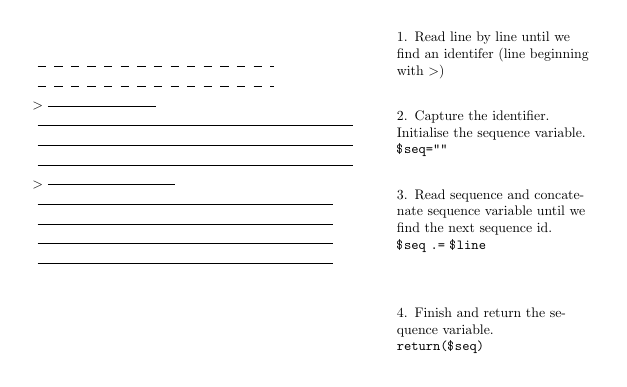
\begin{tikzpicture}[scale=0.5]
      \visible<1->{
\draw [-, dashed] (0, 12) -- (0 + 6, 12);
\draw [-, dashed] (0, 11.5) -- (0 + 6, 11.5);
\node [scale=0.5] (id1) at (0,1	1) {\textgreater};
\draw [-] (id1) -- (0 + 3, 11);
\draw [-] (0, 10.5) -- (0 + 8, 10.5);
\draw [-] (0, 10) -- (0 + 8, 10);
\draw [-] (0, 9.5) -- (0 + 8, 9.5);
\node [scale=0.5] (id2) at (0,9) {\textgreater};
\draw [-] (id2) -- (0 + 3.5, 9);
\draw [-] (0, 8.5) -- (0 + 7.5, 8.5);
\draw [-] (0, 8) -- (0 + 7.5, 8);
\draw [-] (0, 7.5) -- (0 + 7.5, 7.5);
\draw [-] (0, 7) -- (0 + 7.5, 7);
}

\visible<2->{
\node [below right, align=left, text width=5cm, scale=0.5] at (9,13) {1. Read
line by line until
we find an identifer (line beginning with \textgreater)};
}
\visible<3->{
\node [below right, align=left, text width=5cm, scale=0.5] at (9,11) {2. Capture
the identifier.\\Initialise the sequence variable.\\\texttt{\$seq=""}};
}
\visible<4->{
\node [below right, align=left, text width=5cm, scale=0.5] at (9,9) {3. Read
sequence and concatenate sequence variable until we find the next sequence
id.\\\texttt{\$seq .= \$line}};
\node [below right, align=left, text width=5cm, scale=0.5] at (9,6) {4. Finish and
return the sequence variable.\\\texttt{return(\$seq)}};
}



    \end{tikzpicture}
  \end{figure}

\end{frame}

\begin{frame}[fragile]{Read sequence, the code}
  Store sequence in scalar strings; then the read function should simply
  return the string:
  
  \begin{perlcode}
    sub read_fasta {
      ## reads a single sequence from a fasta file
      my $seqFile = shift @_;
      my $seq = "";
      open(my $in, "<", $seqFile) or die "unable to open $seqFile $!\n";
      my $found_identifier = 0;
      while(<$in>){
        chomp;
        if($_ =~ /^>\S+/ ){
          if($found_identifier){
            last;
          }else{
            $found_identifier = 1;
            next;
          }
        }
        if($found_identifier){
          $seq .= $_;
        }
      return( $seq );
    }
  \end{perlcode}
  
\end{frame}

\begin{frame}[fragile]{Read sequences}
  To use this function (\texttt{read\_fasta}) simply put the function
  definition at the end of the file and call the function:

  \begin{perlcode}
    #!/usr/bin/perl 
    use warnings;
    
    ($seqFile1, $seqFile2) = @ARGV;
    
    $seq1 = read_fasta( $seqFile1 );
    $seq2 = read_fasta( $seqFile 2);
    
    ## then make use of $seq1 and $seq2 here...

    sub read_fasta {
      ## reads a single sequence from a fasta file
      ## etc...
    }
  \end{perlcode}
\end{frame}


\begin{frame}[fragile]{Read the substitution matrix}
  Store the matrix as a two dimensional hash:

  \verb|$matrix{ $aa1 }{ $aa2 }|
  
  \begin{figure}[ht]
    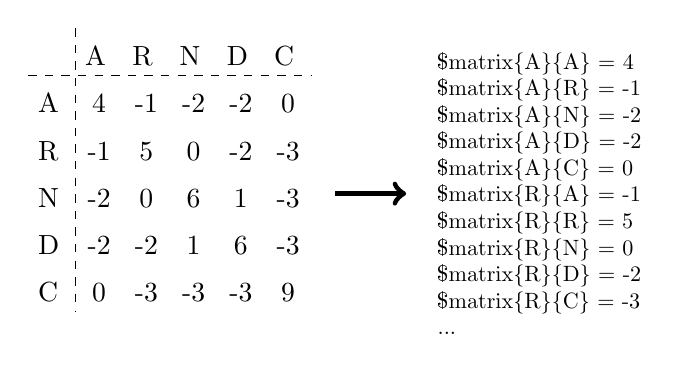
\begin{tikzpicture}[scale=0.5]
      \node [above right] at (1.2,10) {A};
\node [above right] at (0,8.8) {A};
\node [above right] at (2.4,10) {R};
\node [above right] at (0,7.6) {R};
\node [above right] at (3.6,10) {N};
\node [above right] at (0,6.4) {N};
\node [above right] at (4.8,10) {D};
\node [above right] at (0,5.2) {D};
\node [above right] at (6,10) {C};
\node [above right] at (0,4) {C};
\draw [dashed, -] (0,10) -- (7.2,10);
\draw [dashed, -] (1.2,11.2) -- (1.2, 4);
\node [above] at (1.8,8.8) {4};
\node [above] at (3,8.8) {-1};
\node [above] at (4.2,8.8) {-2};
\node [above] at (5.4,8.8) {-2};
\node [above] at (6.6,8.8) {0};
\node [above] at (1.8,7.6) {-1};
\node [above] at (3,7.6) {5};
\node [above] at (4.2,7.6) {0};
\node [above] at (5.4,7.6) {-2};
\node [above] at (6.6,7.6) {-3};
\node [above] at (1.8,6.4) {-2};
\node [above] at (3,6.4) {0};
\node [above] at (4.2,6.4) {6};
\node [above] at (5.4,6.4) {1};
\node [above] at (6.6,6.4) {-3};
\node [above] at (1.8,5.2) {-2};
\node [above] at (3,5.2) {-2};
\node [above] at (4.2,5.2) {1};
\node [above] at (5.4,5.2) {6};
\node [above] at (6.6,5.2) {-3};
\node [above] at (1.8,4) {0};
\node [above] at (3,4) {-3};
\node [above] at (4.2,4) {-3};
\node [above] at (5.4,4) {-3};
\node [above] at (6.6,4) {9};
\visible<2->{
\draw [->, line width=2] (7.8,7) -- (9.6,7);
\node [right, align=left, scale=0.8] at (10.2,7) {  \$matrix\{A\}\{A\} = 4\\
\$matrix\{A\}\{R\} = -1\\ \$matrix\{A\}\{N\} = -2\\ \$matrix\{A\}\{D\} = -2\\
\$matrix\{A\}\{C\} = 0\\ \$matrix\{R\}\{A\} = -1\\ \$matrix\{R\}\{R\} = 5\\
\$matrix\{R\}\{N\} = 0\\ \$matrix\{R\}\{D\} = -2\\ \$matrix\{R\}\{C\} = -3\\...};

}

    \end{tikzpicture}
  \end{figure}

\end{frame}

\begin{frame}[fragile]{Read the substitution matrix (2)}
  \begin{enumerate}
  \item Read the first line:
    \begin{enumerate}
    \item Split the line on spaces $\rightarrow$ array of letters called
      \texttt{@aa2}.
      \pause
    \item Remove the first entry in the array as it contains a space
      (\texttt{shift}).\\
      \pause
      $\rightarrow$ \verb|@aa2 = (A, R, N, D, C)|
    \end{enumerate}
    \pause
  \item Read each line at a time:
    \begin{enumerate}
    \item Split the line on spaces $\rightarrow$ array of letters called
      \texttt{@tmp}.\\
      \pause
      $\rightarrow$ \verb|@tmp = (A, 4, -1, -2, -2, 0)|
      \pause
    \item Use \texttt{shift} to remove the first element in the array and
      assign it to \verb|$aa1|.\\
      \pause
      $\rightarrow$ \verb|$aa1 = A|\\
      $\rightarrow$ \verb|@tmp = (4, -1, -2, -2, 0)|\\
      \pause
    \item Go through each element in \verb|@tmp|, by setting the value of
      \verb|$i| from 0 to \verb|$#tmp|. Assign values to 
      the \verb|%matrix| hash:\\
      \verb|$matrix{$aa1}{ $aa2[$i] } = $tmp[$i]|
    \end{enumerate}
  \end{enumerate}
\end{frame}

\begin{frame}[fragile]{a matrix read function}
  \begin{perlcode}
    sub read_matrix{
      my $mfile = shift @_;
      my %matrix = ();
      open(my $in, "<", $mfile) or die "unable to open $mfile $!\n";
      my $header_line = <$in>;
      chomp $header_line;
      my @aa2 = split /\s+/, $header_line;
      shift @aa2;
      while(<$in>){
        chomp;
        my @tmp = split /\s+/, $_;
        my $aa1 = shift @tmp;
        for my $i(0..$#tmp){
          $matrix{$aa1}{$aa2[$i]} = $tmp[$i];
        }
      }
      return(matrix);
    }
  \end{perlcode}

  like we did last week!
\end{frame}

\begin{frame}[fragile]{Read sequences and matrix}
  Again to use the function, put it at the end of the file and call it with
  the name of a file containing the matrix that you want to use:

  \begin{perlcode}
    #!/usr/bin/perl 
    use warnings;
    
    ($seqFile1, $seqFile2, $matriFile) = @ARGV;
    
    $seq1 = read_fasta( $seqFile1 );
    $seq2 = read_fasta( $seqFile2);
    
    %matrix = read_matrix($matrixFile);

    ## then make use of $seq1 and $seq2 here...

    sub read_matrix{
      my $mfile = shift @_;
      ## etc..
    }

    sub read_fasta {
      ## reads a single sequence from a fasta file
      ## etc...
    }
  \end{perlcode}
\end{frame}

\begin{frame}[fragile]{Calculate an alignment score}
  \begin{figure}[ht]
    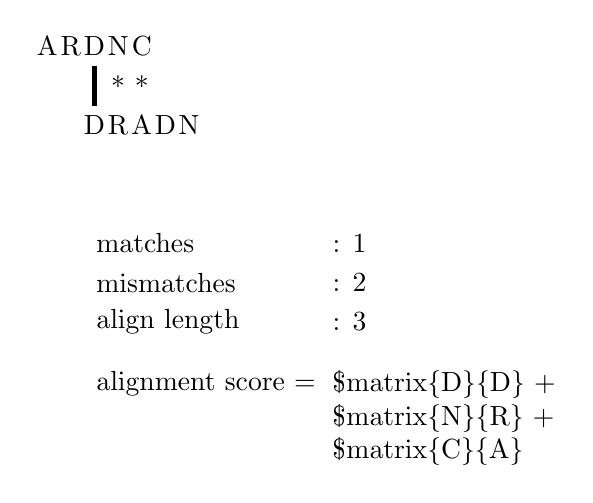
\begin{tikzpicture}[scale=0.5]
      	\node  [] (a0) at (0 + 0, 15) {A};
	\node  [] (a1) at (0 + 0.6, 15) {R};
	\node  [] (a2) at (0 + 1.2, 15) {D};
	\node  [] (a3) at (0 + 1.8, 15) {N};
	\node  [] (a4) at (0 + 2.4, 15) {C};
	\node [] (b0) at (1.2,13) {D};
	\draw [line width=2, -] (a2) -- (b0);
	\node [] (b1) at (1.8,13) {R};
	\node at (1.8,14) {*};
	\node [] (b2) at (2.4,13) {A};
	\node at (2.4,14) {*};
	\node [] (b3) at (3,13) {D};
	\node [] (b4) at (3.6,13) {N};
	\node [right] at (1,10) {matches};
	\node [right] at (7,10) {: 1};
	\node [right] at (1,9) {mismatches};
	\node [right] at (7,9) {: 2};
	\node [right] at (1,8) {align length};
	\node [right] at (7,8) {: 3};
	\node [below right] at (1, 7) {alignment score =};
	\node [below right, align=left] at (7,7) { \$matrix\{D\}\{D\} +\\ \$matrix\{N\}\{R\} +\\ \$matrix\{C\}\{A\} };

    \end{tikzpicture}
  \end{figure}
\end{frame}

\begin{frame}[fragile]{The offsets?}
  \begin{figure}[ht]
    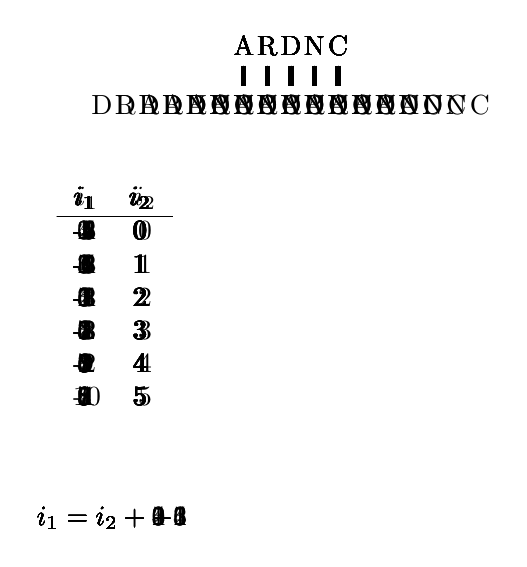
\begin{tikzpicture}[scale=0.5]
      \visible<1>{
	\node  [] (a0) at (0 + 0, 15) {A};
	\node  [] (a1) at (0 + 0.6, 15) {R};
	\node  [] (a2) at (0 + 1.2, 15) {D};
	\node  [] (a3) at (0 + 1.8, 15) {N};
	\node  [] (a4) at (0 + 2.4, 15) {C};
	\node [] (b0) at (-3.6,13.5) {D};
	\node [] (b1) at (-3,13.5) {R};
	\node [] (b2) at (-2.4,13.5) {A};
	\node [] (b3) at (-1.8,13.5) {D};
	\node [] (b4) at (-1.2,13.5) {N};
	\node [] (b5) at (-0.6,13.5) {C};
	\node [right] at (-5,9) { \begin{tabular}{cc}\\
$i_1$ & $i_2$ \\
\hline
-6 & 0 \\
-5 & 1 \\
-4 & 2 \\
-3 & 3 \\
-2 & 4 \\
-1 & 5 \\
\end{tabular}
 };
	\node [right] at (-5-0.5, 3) { $i_1 = i_2 + -6$ };
}
\visible<2>{
	\node  [] (a0) at (0 + 0, 15) {A};
	\node  [] (a1) at (0 + 0.6, 15) {R};
	\node  [] (a2) at (0 + 1.2, 15) {D};
	\node  [] (a3) at (0 + 1.8, 15) {N};
	\node  [] (a4) at (0 + 2.4, 15) {C};
	\node [] (b0) at (-3,13.5) {D};
	\node [] (b1) at (-2.4,13.5) {R};
	\node [] (b2) at (-1.8,13.5) {A};
	\node [] (b3) at (-1.2,13.5) {D};
	\node [] (b4) at (-0.6,13.5) {N};
	\node [] (b5) at (0,13.5) {C};
	\draw [line width=0.5, -, dotted] (a0) -- (b5);
	\node [right] at (-5,9) { \begin{tabular}{cc}\\
$i_1$ & $i_2$ \\
\hline
-5 & 0 \\
-4 & 1 \\
-3 & 2 \\
-2 & 3 \\
-1 & 4 \\
0 & 5 \\
\end{tabular}
 };
	\node [right] at (-5-0.5, 3) { $i_1 = i_2 + -5$ };
}
\visible<3>{
	\node  [] (a0) at (0 + 0, 15) {A};
	\node  [] (a1) at (0 + 0.6, 15) {R};
	\node  [] (a2) at (0 + 1.2, 15) {D};
	\node  [] (a3) at (0 + 1.8, 15) {N};
	\node  [] (a4) at (0 + 2.4, 15) {C};
	\node [] (b0) at (-2.4,13.5) {D};
	\node [] (b1) at (-1.8,13.5) {R};
	\node [] (b2) at (-1.2,13.5) {A};
	\node [] (b3) at (-0.6,13.5) {D};
	\node [] (b4) at (0,13.5) {N};
	\draw [line width=0.5, -, dotted] (a0) -- (b4);
	\node [] (b5) at (0.6,13.5) {C};
	\draw [line width=0.5, -, dotted] (a1) -- (b5);
	\node [right] at (-5,9) { \begin{tabular}{cc}\\
$i_1$ & $i_2$ \\
\hline
-4 & 0 \\
-3 & 1 \\
-2 & 2 \\
-1 & 3 \\
0 & 4 \\
1 & 5 \\
\end{tabular}
 };
	\node [right] at (-5-0.5, 3) { $i_1 = i_2 + -4$ };
}
\visible<4>{
	\node  [] (a0) at (0 + 0, 15) {A};
	\node  [] (a1) at (0 + 0.6, 15) {R};
	\node  [] (a2) at (0 + 1.2, 15) {D};
	\node  [] (a3) at (0 + 1.8, 15) {N};
	\node  [] (a4) at (0 + 2.4, 15) {C};
	\node [] (b0) at (-1.8,13.5) {D};
	\node [] (b1) at (-1.2,13.5) {R};
	\node [] (b2) at (-0.6,13.5) {A};
	\node [] (b3) at (0,13.5) {D};
	\draw [line width=0.5, -, dotted] (a0) -- (b3);
	\node [] (b4) at (0.6,13.5) {N};
	\draw [line width=0.5, -, dotted] (a1) -- (b4);
	\node [] (b5) at (1.2,13.5) {C};
	\draw [line width=0.5, -, dotted] (a2) -- (b5);
	\node [right] at (-5,9) { \begin{tabular}{cc}\\
$i_1$ & $i_2$ \\
\hline
-3 & 0 \\
-2 & 1 \\
-1 & 2 \\
0 & 3 \\
1 & 4 \\
2 & 5 \\
\end{tabular}
 };
	\node [right] at (-5-0.5, 3) { $i_1 = i_2 + -3$ };
}
\visible<5>{
	\node  [] (a0) at (0 + 0, 15) {A};
	\node  [] (a1) at (0 + 0.6, 15) {R};
	\node  [] (a2) at (0 + 1.2, 15) {D};
	\node  [] (a3) at (0 + 1.8, 15) {N};
	\node  [] (a4) at (0 + 2.4, 15) {C};
	\node [] (b0) at (-1.2,13.5) {D};
	\node [] (b1) at (-0.6,13.5) {R};
	\node [] (b2) at (0,13.5) {A};
	\draw [line width=2, -] (a0) -- (b2);
	\node [] (b3) at (0.6,13.5) {D};
	\draw [line width=0.5, -, dotted] (a1) -- (b3);
	\node [] (b4) at (1.2,13.5) {N};
	\draw [line width=0.5, -, dotted] (a2) -- (b4);
	\node [] (b5) at (1.8,13.5) {C};
	\draw [line width=0.5, -, dotted] (a3) -- (b5);
	\node [right] at (-5,9) { \begin{tabular}{cc}\\
$i_1$ & $i_2$ \\
\hline
-2 & 0 \\
-1 & 1 \\
0 & 2 \\
1 & 3 \\
2 & 4 \\
3 & 5 \\
\end{tabular}
 };
	\node [right] at (-5-0.5, 3) { $i_1 = i_2 + -2$ };
}
\visible<6>{
	\node  [] (a0) at (0 + 0, 15) {A};
	\node  [] (a1) at (0 + 0.6, 15) {R};
	\node  [] (a2) at (0 + 1.2, 15) {D};
	\node  [] (a3) at (0 + 1.8, 15) {N};
	\node  [] (a4) at (0 + 2.4, 15) {C};
	\node [] (b0) at (-0.6,13.5) {D};
	\node [] (b1) at (0,13.5) {R};
	\draw [line width=0.5, -, dotted] (a0) -- (b1);
	\node [] (b2) at (0.6,13.5) {A};
	\draw [line width=0.5, -, dotted] (a1) -- (b2);
	\node [] (b3) at (1.2,13.5) {D};
	\draw [line width=2, -] (a2) -- (b3);
	\node [] (b4) at (1.8,13.5) {N};
	\draw [line width=2, -] (a3) -- (b4);
	\node [] (b5) at (2.4,13.5) {C};
	\draw [line width=2, -] (a4) -- (b5);
	\node [right] at (-5,9) { \begin{tabular}{cc}\\
$i_1$ & $i_2$ \\
\hline
-1 & 0 \\
0 & 1 \\
1 & 2 \\
2 & 3 \\
3 & 4 \\
4 & 5 \\
\end{tabular}
 };
	\node [right] at (-5-0.5, 3) { $i_1 = i_2 + -1$ };
}
\visible<7>{
	\node  [] (a0) at (0 + 0, 15) {A};
	\node  [] (a1) at (0 + 0.6, 15) {R};
	\node  [] (a2) at (0 + 1.2, 15) {D};
	\node  [] (a3) at (0 + 1.8, 15) {N};
	\node  [] (a4) at (0 + 2.4, 15) {C};
	\node [] (b0) at (0,13.5) {D};
	\draw [line width=0.5, -, dotted] (a0) -- (b0);
	\node [] (b1) at (0.6,13.5) {R};
	\draw [line width=2, -] (a1) -- (b1);
	\node [] (b2) at (1.2,13.5) {A};
	\draw [line width=0.5, -, dotted] (a2) -- (b2);
	\node [] (b3) at (1.8,13.5) {D};
	\draw [line width=0.5, -, dotted] (a3) -- (b3);
	\node [] (b4) at (2.4,13.5) {N};
	\draw [line width=0.5, -, dotted] (a4) -- (b4);
	\node [] (b5) at (3,13.5) {C};
	\node [right] at (-5,9) { \begin{tabular}{cc}\\
$i_1$ & $i_2$ \\
\hline
0 & 0 \\
1 & 1 \\
2 & 2 \\
3 & 3 \\
4 & 4 \\
5 & 5 \\
\end{tabular}
 };
	\node [right] at (-5-0.5, 3) { $i_1 = i_2 + 0$ };
}
\visible<8>{
	\node  [] (a0) at (0 + 0, 15) {A};
	\node  [] (a1) at (0 + 0.6, 15) {R};
	\node  [] (a2) at (0 + 1.2, 15) {D};
	\node  [] (a3) at (0 + 1.8, 15) {N};
	\node  [] (a4) at (0 + 2.4, 15) {C};
	\node [] (b0) at (0.6,13.5) {D};
	\draw [line width=0.5, -, dotted] (a1) -- (b0);
	\node [] (b1) at (1.2,13.5) {R};
	\draw [line width=0.5, -, dotted] (a2) -- (b1);
	\node [] (b2) at (1.8,13.5) {A};
	\draw [line width=0.5, -, dotted] (a3) -- (b2);
	\node [] (b3) at (2.4,13.5) {D};
	\draw [line width=0.5, -, dotted] (a4) -- (b3);
	\node [] (b4) at (3,13.5) {N};
	\node [] (b5) at (3.6,13.5) {C};
	\node [right] at (-5,9) { \begin{tabular}{cc}\\
$i_1$ & $i_2$ \\
\hline
1 & 0 \\
2 & 1 \\
3 & 2 \\
4 & 3 \\
5 & 4 \\
6 & 5 \\
\end{tabular}
 };
	\node [right] at (-5-0.5, 3) { $i_1 = i_2 + 1$ };
}
\visible<9>{
	\node  [] (a0) at (0 + 0, 15) {A};
	\node  [] (a1) at (0 + 0.6, 15) {R};
	\node  [] (a2) at (0 + 1.2, 15) {D};
	\node  [] (a3) at (0 + 1.8, 15) {N};
	\node  [] (a4) at (0 + 2.4, 15) {C};
	\node [] (b0) at (1.2,13.5) {D};
	\draw [line width=2, -] (a2) -- (b0);
	\node [] (b1) at (1.8,13.5) {R};
	\draw [line width=0.5, -, dotted] (a3) -- (b1);
	\node [] (b2) at (2.4,13.5) {A};
	\draw [line width=0.5, -, dotted] (a4) -- (b2);
	\node [] (b3) at (3,13.5) {D};
	\node [] (b4) at (3.6,13.5) {N};
	\node [] (b5) at (4.2,13.5) {C};
	\node [right] at (-5,9) { \begin{tabular}{cc}\\
$i_1$ & $i_2$ \\
\hline
2 & 0 \\
3 & 1 \\
4 & 2 \\
5 & 3 \\
6 & 4 \\
7 & 5 \\
\end{tabular}
 };
	\node [right] at (-5-0.5, 3) { $i_1 = i_2 + 2$ };
}
\visible<10>{
	\node  [] (a0) at (0 + 0, 15) {A};
	\node  [] (a1) at (0 + 0.6, 15) {R};
	\node  [] (a2) at (0 + 1.2, 15) {D};
	\node  [] (a3) at (0 + 1.8, 15) {N};
	\node  [] (a4) at (0 + 2.4, 15) {C};
	\node [] (b0) at (1.8,13.5) {D};
	\draw [line width=0.5, -, dotted] (a3) -- (b0);
	\node [] (b1) at (2.4,13.5) {R};
	\draw [line width=0.5, -, dotted] (a4) -- (b1);
	\node [] (b2) at (3,13.5) {A};
	\node [] (b3) at (3.6,13.5) {D};
	\node [] (b4) at (4.2,13.5) {N};
	\node [] (b5) at (4.8,13.5) {C};
	\node [right] at (-5,9) { \begin{tabular}{cc}\\
$i_1$ & $i_2$ \\
\hline
3 & 0 \\
4 & 1 \\
5 & 2 \\
6 & 3 \\
7 & 4 \\
8 & 5 \\
\end{tabular}
 };
	\node [right] at (-5-0.5, 3) { $i_1 = i_2 + 3$ };
}
\visible<11>{
	\node  [] (a0) at (0 + 0, 15) {A};
	\node  [] (a1) at (0 + 0.6, 15) {R};
	\node  [] (a2) at (0 + 1.2, 15) {D};
	\node  [] (a3) at (0 + 1.8, 15) {N};
	\node  [] (a4) at (0 + 2.4, 15) {C};
	\node [] (b0) at (2.4,13.5) {D};
	\draw [line width=0.5, -, dotted] (a4) -- (b0);
	\node [] (b1) at (3,13.5) {R};
	\node [] (b2) at (3.6,13.5) {A};
	\node [] (b3) at (4.2,13.5) {D};
	\node [] (b4) at (4.8,13.5) {N};
	\node [] (b5) at (5.4,13.5) {C};
	\node [right] at (-5,9) { \begin{tabular}{cc}\\
$i_1$ & $i_2$ \\
\hline
4 & 0 \\
5 & 1 \\
6 & 2 \\
7 & 3 \\
8 & 4 \\
9 & 5 \\
\end{tabular}
 };
	\node [right] at (-5-0.5, 3) { $i_1 = i_2 + 4$ };
}
\visible<12>{
	\node  [] (a0) at (0 + 0, 15) {A};
	\node  [] (a1) at (0 + 0.6, 15) {R};
	\node  [] (a2) at (0 + 1.2, 15) {D};
	\node  [] (a3) at (0 + 1.8, 15) {N};
	\node  [] (a4) at (0 + 2.4, 15) {C};
	\node [] (b0) at (3,13.5) {D};
	\node [] (b1) at (3.6,13.5) {R};
	\node [] (b2) at (4.2,13.5) {A};
	\node [] (b3) at (4.8,13.5) {D};
	\node [] (b4) at (5.4,13.5) {N};
	\node [] (b5) at (6,13.5) {C};
	\node [right] at (-5,9) { \begin{tabular}{cc}\\
$i_1$ & $i_2$ \\
\hline
5 & 0 \\
6 & 1 \\
7 & 2 \\
8 & 3 \\
9 & 4 \\
10 & 5 \\
\end{tabular}
 };
	\node [right] at (-5-0.5, 3) { $i_1 = i_2 + 5$ };
}

    \end{tikzpicture}
  \end{figure}
  \pause
  The offsets run from -length(seq1) $\rightarrow$ length(seq2);
\end{frame}

\begin{frame}[fragile]{offset alignment scores}
  \small {
  The offset alignment score function needs to take four arguments:
  \begin{enumerate}
  \item The two sequences
  \item The offset to use for the alignment
  \item The substitution matrix
  \end{enumerate}
  
  That's three scalars and one hash. To pass the hash we must pass it as a
  reference and then dereference it in the alignment section.
}
  \pause

  \begin{perlcode}
    $score = offset_alignment($seq1, $seq2, $offset, \%matrix);
  \end{perlcode}
\footnotesize {
  To pass as a reference put a \verb|\| in front of the identifier
  \pause

  In the function we can dereference using the \verb|->| operator.
}
  \begin{perlcode}
    sub offset_alignment {
      my ($seq1, $seq2, $offset, $matrix_ref) = @_;
      ## to get the value for a specific pair of amino acids:
      $matrix_ref->{A}{R};
    }
  \end{perlcode}
\end{frame}

\begin{frame}[fragile]{the offset alignment function}
  \begin{perlcode}
    sub offset_align_score {
      my ($seq1, $seq2, $offset, $m_ref) = @_;
      my $score = 0;
      for(my $i=0; $i < length($seq2); $i++){
        my $j = $i + $offset;
        if($j >= 0 && $j < length($seq1)){
          $score += $m_ref->{ substr($seq1, $j, 1) }{ substr($seq2, $i, 1) };
        }
      }
      return( $score );
    }
  \end{perlcode}

  Here we use \texttt{substr()} to avoid splitting the string to an array many
  times.
\end{frame}

\begin{frame}[fragile]{putting all together}
  \begin{perlcode}
    #!/usr/bin/perl -w
    ($seqFile1, $seqFile2, $matrixFile) = @ARGV;
    
    $seq1 = read_fasta( $seqFile1 );
    $seq2 = read_fasta( $seqFile2 );
    %matrix = read_matrix( $matrixFile );
    
    ## we need to use offsets from -length(seq1) to length(seq2)
    ## we can easily loop.. 
    for $offset( -length($seq1)..length($seq2) ){
      $score = offset_align_score( $seq1, $seq2, $offset, \%matrix );
      print "$i\t$score\n";
    }

    ## the function definitions (abbreviated)
    sub read_fasta {
      ####
    }
    sub read_matrix {
      ####
    }
    sub offset_align_score {
      ###
    }
  \end{perlcode}
\end{frame}

\begin{frame}[fragile]{Improvements?}
  \begin{itemize}
  \item That will only print out the offsets and their associated scores;
    might be nice to print out the alignments as well.
  \item This gives scores for global alignments (without gap penalties),
    finding local alignments seems more reasonable.
  \item Use an index rather than this ugly method (which has a complexity of
    $l_2 * (l_1 + l_2)$ where $l_1$ and $l_2$ are the lengths of sequence
    1 and 2 respectively.
  \item Do something like blast; i.e. extend locally matching pairs identifed
    from an index.
  \end{itemize}
\end{frame}

\end{document}
